\noindent In diesem Kapitel wird auf die Analyse bestimmter Schlagwörter in den E-Mails eingegangen. Um diese Analyse durchzuführen habe ich im Internet nach gängigen Wörtern gesucht, die auf eine Spam-Mail hinweisen \cite{Heise.07.06.2021}. Anhand der gefundenen Wörter habe ich passende ausgesucht und als Liste in einem Python Skript hinterlegt. Diese Liste ist in Abbildung \ref{fig:spamwortliste} zu sehen und enthält 176 Schlagwörter. Dabei wurden Kategorien wie Finanzen, Glücksspiel, Gesundheit, Shopping, Dating und Sonstige betrachtet. Für die Analyse der Wörter wurde die .csv-Datei verwendet, welche beim Parsen der .pst-Datei entstanden ist. Diese wurde dann mit je einem Wort aus der Spamwort-Liste durchlaufen und ein Counter erhöht, sobald ein Treffer erzielt wurde. Anschließend wurde die Liste \glqq{}word\_list\grqq{} mit den Headern \glqq{}SpamWords\grqq{} und \glqq{}Hits\grqq{} in eine .csv-Datei exportiert um eine grafische Auswertung dieser Daten vorzunehmen. Der hierfür verwendete Python Code ist in Abbildung \ref{fig:spamwordsearch} zu sehen. Die hierdurch erstellte .csv-Datei habe ich im Anschluss in Microsoft Excel importiert und dort eine Graphische Auswertung durchgeführt. Excel habe ich gewählt, da ich, anders als bei der Auswertung der zeitlichen Eigenschaften der E-Mails, eine andere Art der grafischen Auswertung abseits von Python ausprobieren wollte. \smallskip

\noindent Das Ergebnis der Auswertung ist in Abbildung \ref{fig:spamwortlistegreater100} zu sehen. Am häufigsten kamen davon das Wort \glqq{}Angebot\grqq{} mit 5092 Treffern, danach \glqq{}Date\grqq{} mit 2991 Treffern gefolgt von \glqq{}klicken\grqq{} mit 1319 Treffern vor. Diese Wörter sind in die Kategorien Shopping und Dating sowie Sonstige einzuordnen. In der Abbildung \ref{fig:spamwortlistegreater100} sind alle Wörter mit einer Trefferanzahl von mehr als 100 abgebildet. Im zweiten Datensatz wurden ebenfalls alle Wörter mit mehr als 100 Treffern abgebildet (\ref{fig:spamwortlistegreater100merged}). Dabei war das Wort \glqq{}Date\grqq{} auch hier sehr oft vertreten und zwar mit 1027 Treffern. Danach folgt das Wort \glqq{}Angebot\grqq{} mit 716 Treffern. Die zwei Wörter mit den höchsten Treffern sind also identisch zum anderen Datensatz. Auf beiden Grafiken zur Auswertung der Spamwortsuche ist auch erkennbar, dass sich die Wörter mit über 100 Treffern überschneiden. Somit lässt sich zumindest anhand dieser beider .pst-Dateien ein Muster an häufig auftretenden Schlagworten erkennen. 

\begin{figure}[!ht]
    \centering
    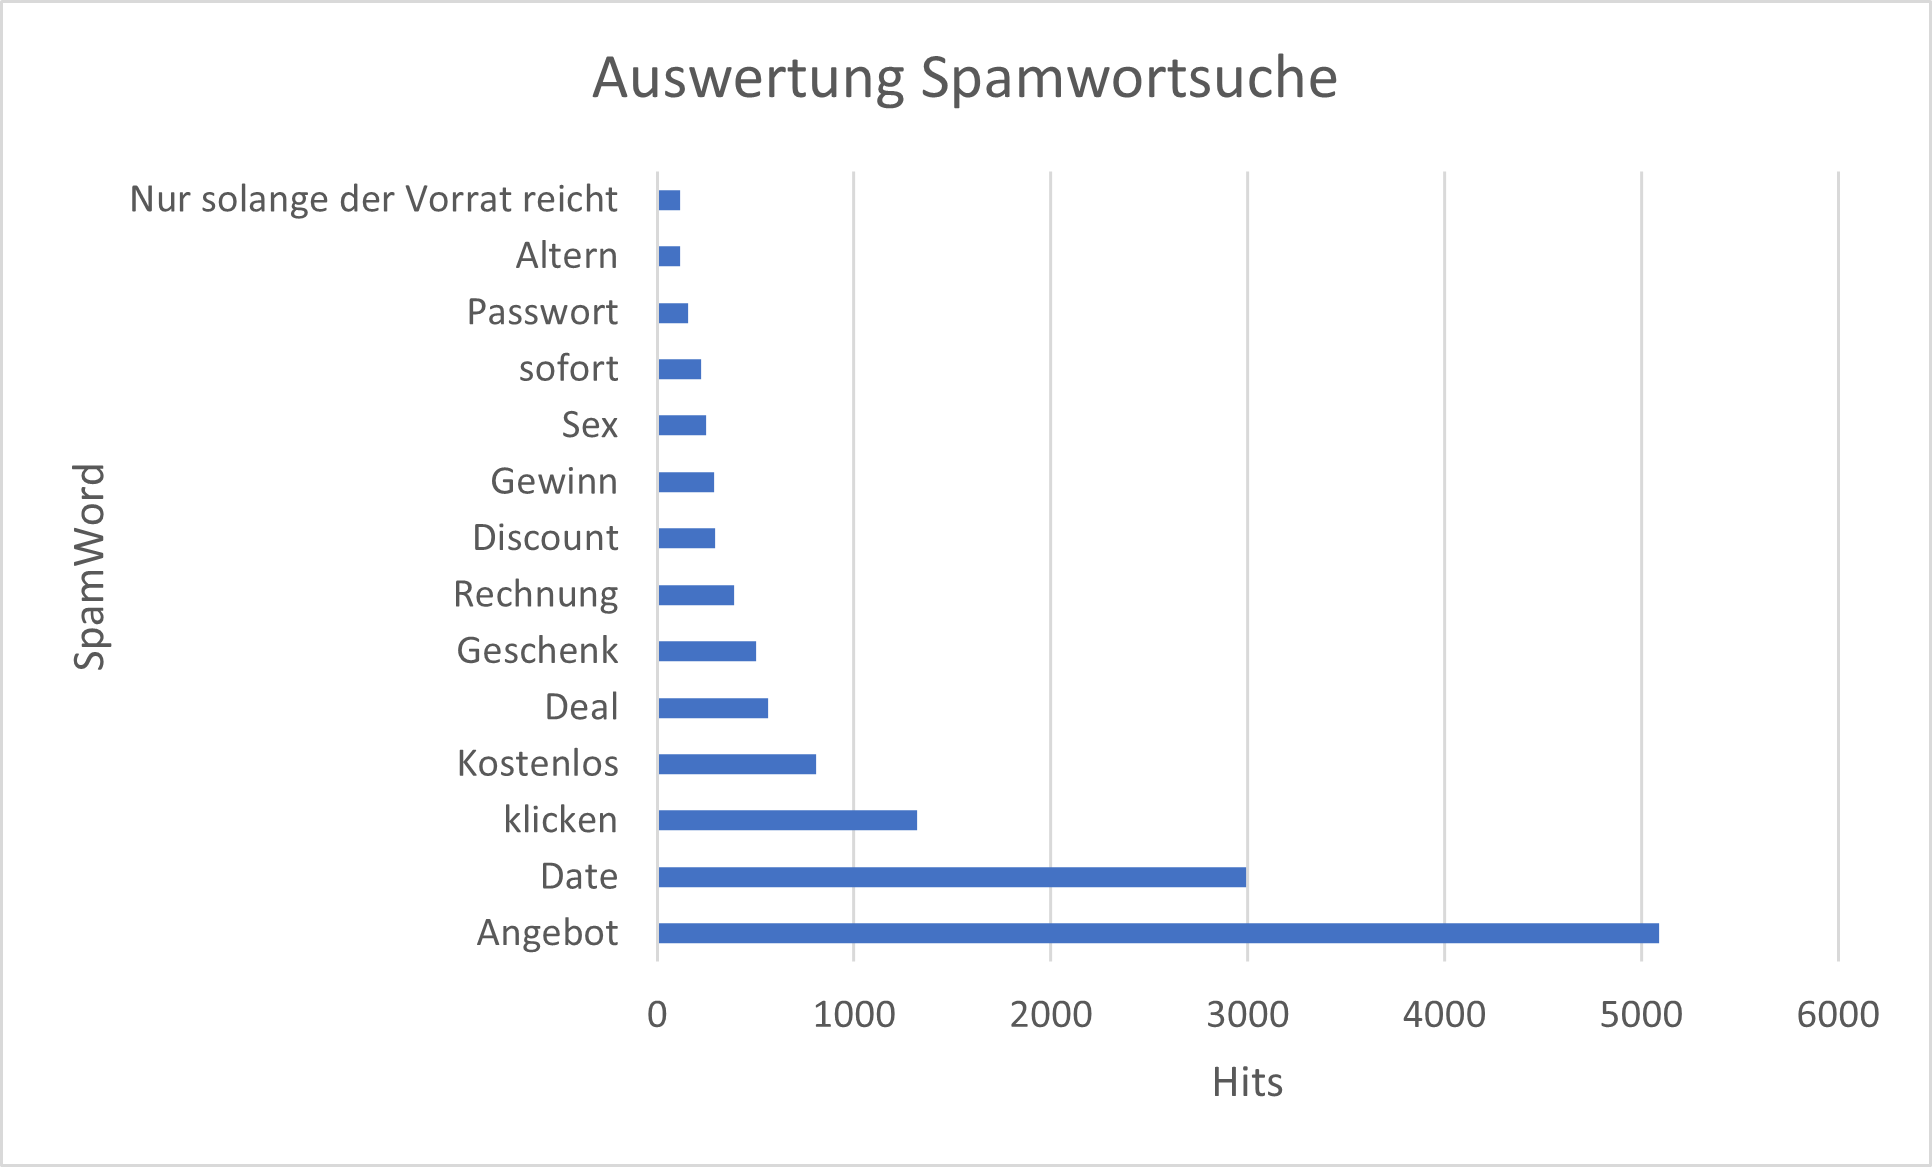
\includegraphics[width=0.75\textwidth]{images/Auswertung_Spamwortsuche.png}
    \caption{Wörter mit mehr als 100 Treffern - Datensatz mit 4102 E-Mails} 
    \label{fig:spamwortlistegreater100}
\end{figure}


\begin{figure}[!ht]
    \centering
    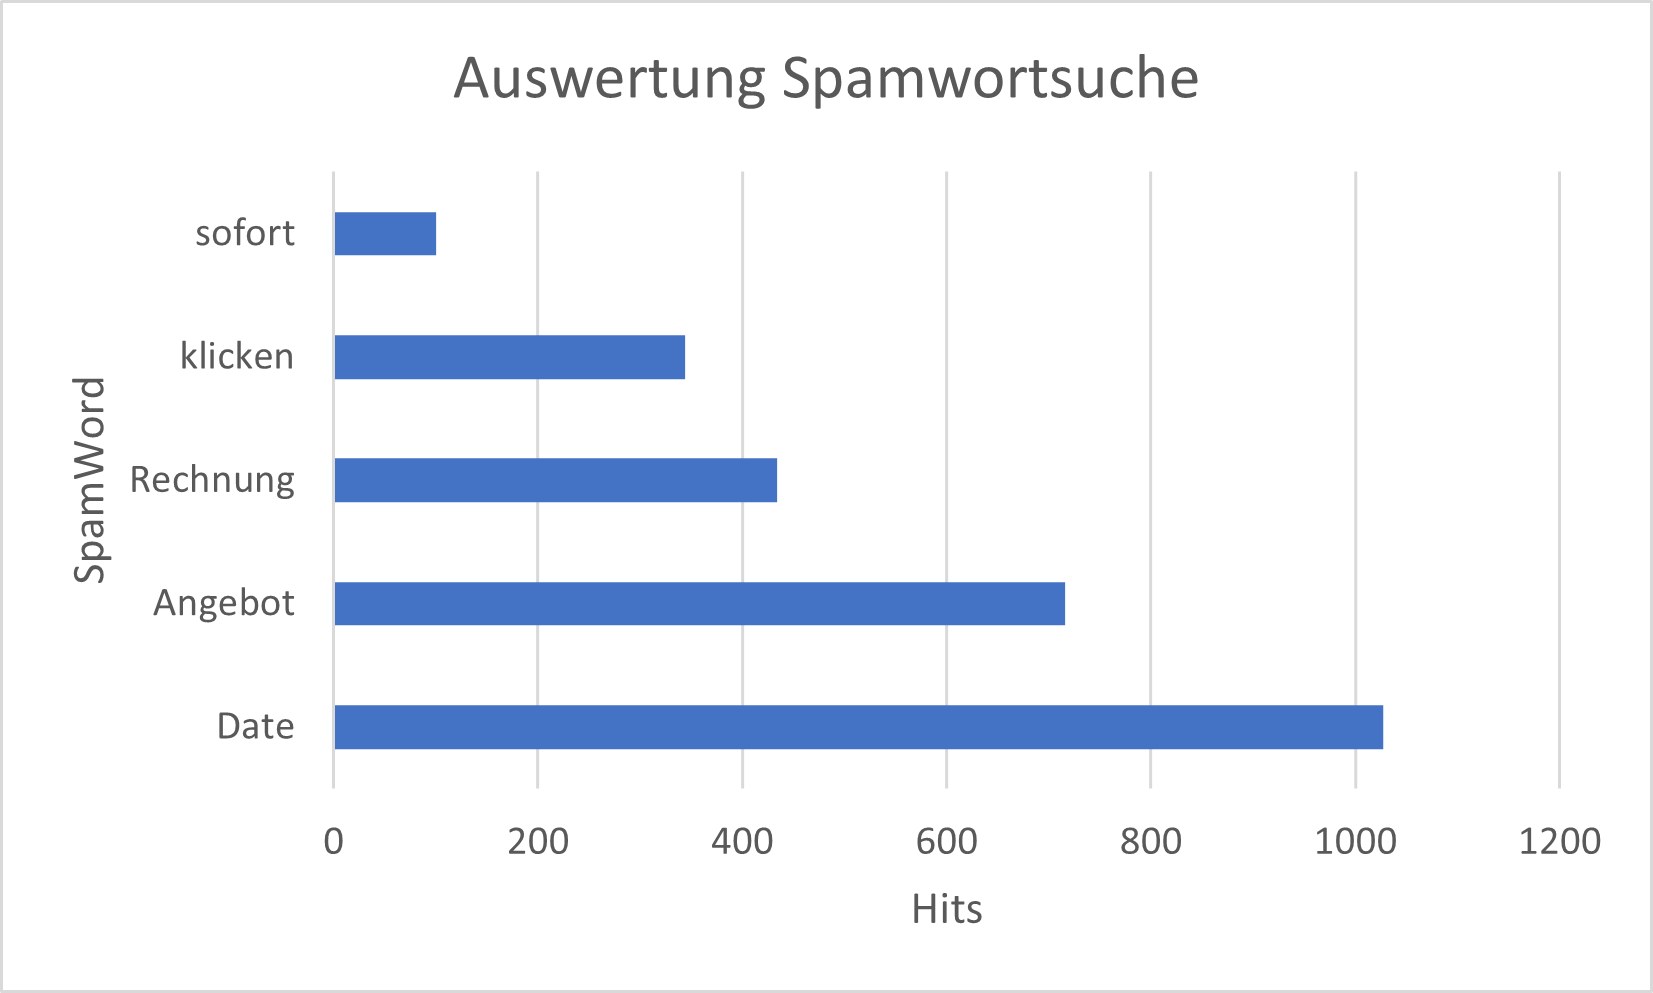
\includegraphics[width=0.75\textwidth]{images/Merged_Auswertung_Spamwortsuche.png}
    \caption{Wörter mit mehr als 100 Treffern - Datensatz mit 6692 E-Mails} 
    \label{fig:spamwortlistegreater100merged}
\end{figure}

\newpage